\documentclass[a4paper,12pt]{book}

\usepackage{url}
\usepackage[brazil]{babel}
\usepackage[pdftex]{graphicx}
\usepackage[pdftex]{hyperref}
\usepackage{float}

\title{Xadrez em Realidade Aumentada - Manual}
\author{
		Douglas Bettioli Barreto (NUSP 6920223)
		\and Giancarlo Rigo (NUSP 6910034)
		\and Rafael Reggiani Manzo (NUSP 6797150)
	   }

\begin{document}

\maketitle

\part{Considera\c c\~oes gerais}
\label{part:consideracoesgerais}
  \chapter{B\'asico}
  \label{chbasico}
  \section{Compila\c c\~ao}
	\label{sec:cgcompilacao}
	Este software foi desenvolvido e testado em Linux Ubuntu 10.04 (32 bits). Mas,
	teoricamente, deve funcionar em qualquer maquina que atenda aos requisitos
	(\ref{subsec:cgrequisitos})
	
	\subsection{Requisitos}
	\label{subsec:cgrequisitos}
	\begin{itemize}
		\item{Adobe Flex Compiler (mxmlc) Version 4.1.0 build 16076}
	\end{itemize}
	
	\subsection{Makefile}
	Encontrado dentro da pasta src. Dentro dele substitua o caminho para o mxmlc do
	seu Flex SDK.
	Existem duas op\c c\~oes de debug:
	\begin{itemize}
	  \item{Compilar a vers\~ao de produ\c c~ao: ``make''}
	  \item{Compilar a vers\~ao de debug: ``make debug''}
	\end{itemize}

\part{Manual do usu\'ario}
\label{part:manualdousuario}
	\chapter{Introdu\c c\~ao}
	Para rodar o programa, o usuário far\'a uso do makefile, arquivo que ser\'a
	utilizado pelo programa make, que ir\'a compilar o programa. Para rodar o make,
	basta acessar o diret\'orio aonde está o arquivo “makefile” pelo terminal e
	digitar make. \'E importante ressaltar que para a identifica\c c\~ao das tags,
	a c\^amera deve ser posicionada com direção vertical \` superf\'cie das tags, preferencialmente em locais com boa iluminação e em superf\'icies planas.

\part{Manual do Desenvolvedor}
\label{part:manualdodesenvolvedor}
	\chapter{Diagrama de classes}
	\label{ch:diagramadeclasses}
	\begin{figure}[H]
	\centering
	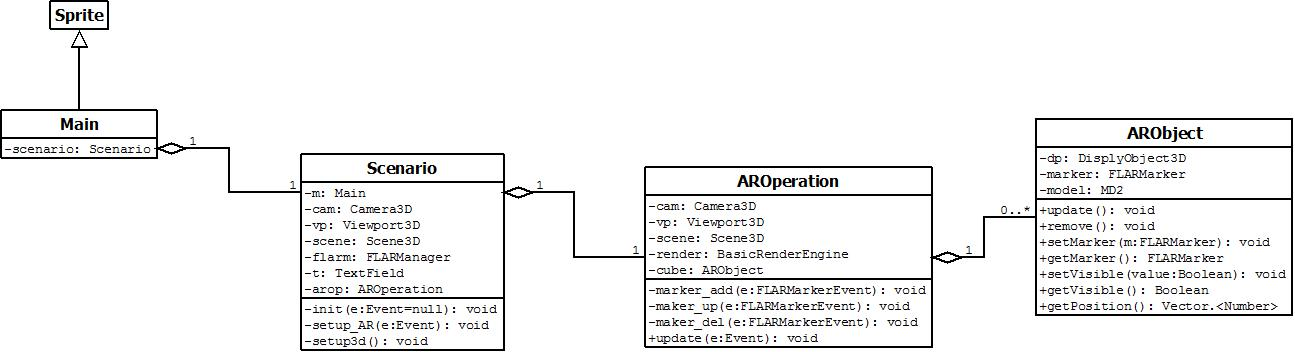
\includegraphics[width=0.7\textwidth, height=0.7\textheight]{diagramadeclasses}
	\end{figure}
	\footnote{Ver observacoes sobre a clase AROperation em
			  \ref{subsec:ecclassearoperation}
			 }

  \chapter{CRC cards}
  \label{ch:crccards}
  \section{Pacote Principal}
	\label{sec:crcpacoteprincipal}
    \subsection{Main}
    \label{subsec:crcmain}
    \begin{figure}[H]
	  \centering
	  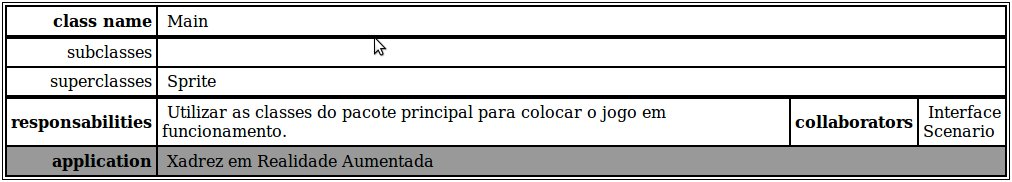
\includegraphics[width=1.0\textwidth]{crc/Main}
	  \end{figure}
  	\subsection{Scenario}
    \label{subsec:crcscenario}
    \begin{figure}[H]
	  \centering
	  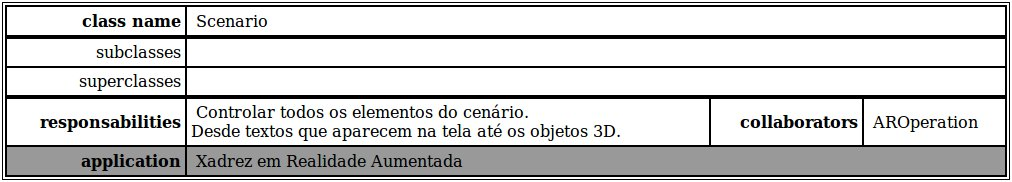
\includegraphics[width=1.0\textwidth]{crc/Scenario}
	  \end{figure}
  \section{Pacote AugmentedReality}
  \label{sec:crcpacoteaugmentedreality}
    \subsection{ARCronometer}
    \label{subsec:crcarcronometer}
    \begin{figure}[H]
	  \centering
	  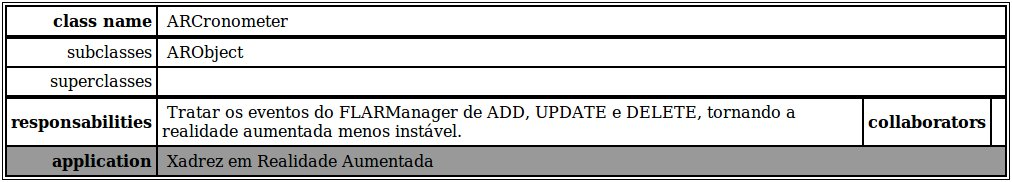
\includegraphics[width=1.0\textwidth]{crc/ARCronometer}
	  \end{figure}
    \subsection{ARObject}
    \label{subsec:crcarobject}
    \begin{figure}[H]
	  \centering
	  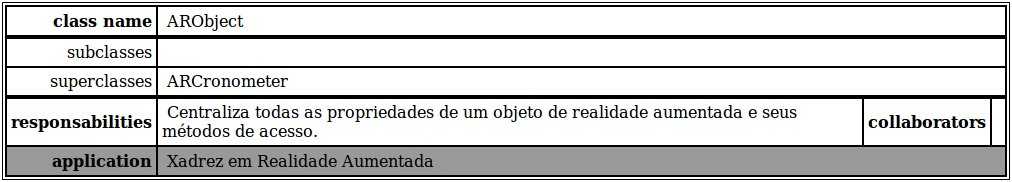
\includegraphics[width=1.0\textwidth]{crc/ARObject}
	  \end{figure}
    \subsection{ARIndependentObject}
    \label{subsec:crcarindependentobject}
    \begin{figure}[H]
	  \centering
	  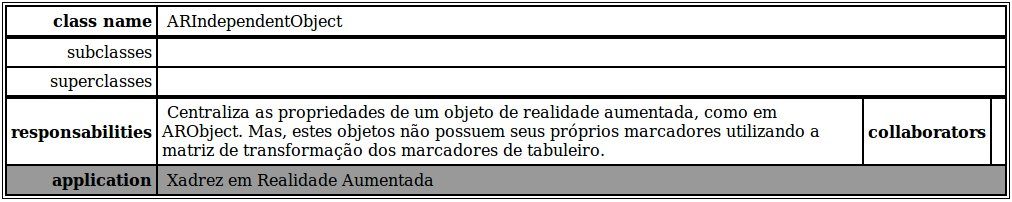
\includegraphics[width=1.0\textwidth]{crc/ARIndependentObject}
	  \end{figure}
    \subsection{AROperation}
    \label{subsec:crcaroperation}
    \begin{figure}[H]
	  \centering
	  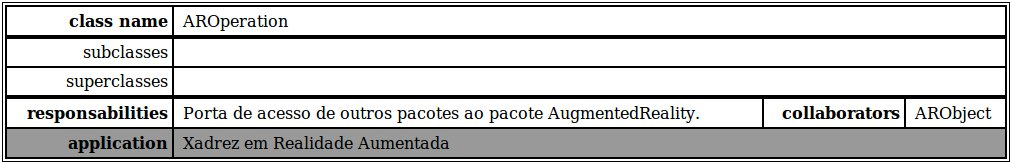
\includegraphics[width=1.0\textwidth]{crc/AROperation}
	  \end{figure}
  \section{Pacote Game}
  \label{sec:crcpacotegame}
    \subsection{PieceType}
    \label{subsec:crcpiecetype}
    \begin{figure}[H]
	  \centering
	  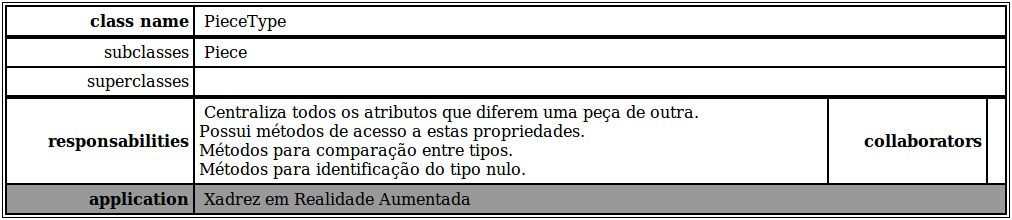
\includegraphics[width=1.0\textwidth]{crc/PieceType}
	  \end{figure}
    \subsection{Piece}
    \label{subsec:crcpiece}
    \begin{figure}[H]
	  \centering
	  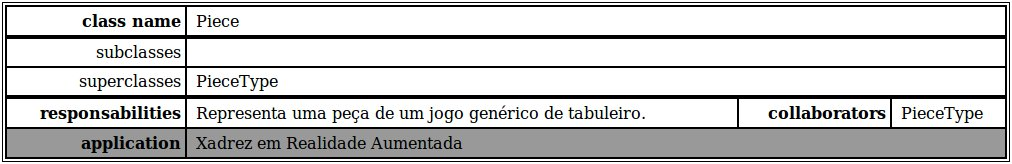
\includegraphics[width=1.0\textwidth]{crc/Piece}
	  \end{figure}
    \subsection{Board}
    \label{subsec:crcboard}
    \begin{figure}[H]
	  \centering
	  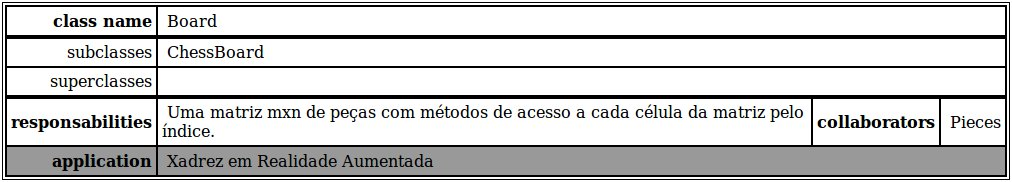
\includegraphics[width=1.0\textwidth]{crc/Board}
	  \end{figure}
    \subsection{Pacote Chess}
    \label{subsec:crcpacotechess}
      \subsection{ChessBoard}
      \label{subsubsec:crcchessboard}
      \begin{figure}[H]
	    \centering
	    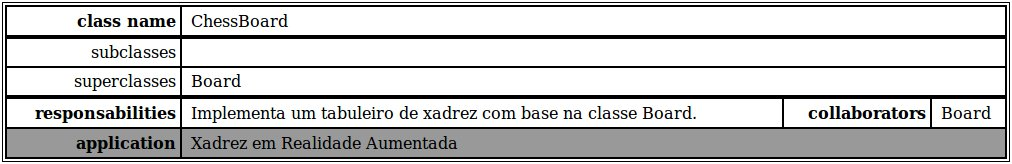
\includegraphics[width=1.0\textwidth]{crc/ChessBoard}
	    \end{figure}
      \subsection{ChessPiece}
      \label{subsubsec:crcchesspiece}
      \begin{figure}[H]
	    \centering
	    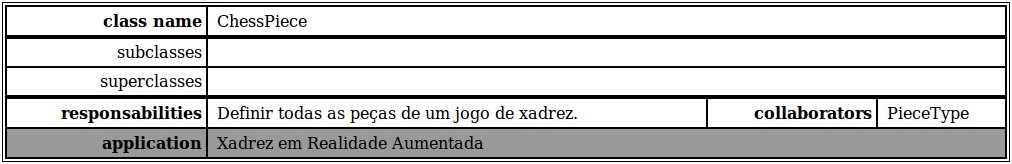
\includegraphics[width=1.0\textwidth]{crc/ChessPieces}
	    \end{figure}
      \subsection{Validator}
      \label{subsec:crcvalidator}
      \begin{figure}[H]
	    \centering
	    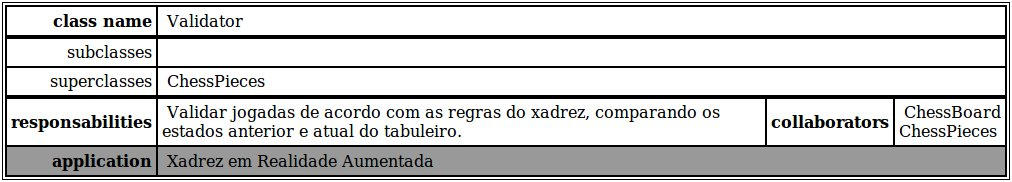
\includegraphics[width=1.0\textwidth]{crc/Validator}
	    \end{figure}

	\chapter{Prova de conceito}
	\label{ch:provadeconceito}
		\section{Introdu\c c\~ao}
		\label{sec:pcintroducao}
		A prova de conceito consistiu em abordar os pontos chave do projeto no que se
		refere a realidade aumentada. Nela, foram tratados temas como o reconhecimento
		de multiplos marcadores e a capacidade de obter as coordenadas do marcador no
		espa\c co. \footnote{A prova de conceito \'e o branch ``12 tags ao mesmo
		tempo" do reposit\'orio}
		
		\section{Marcadores}
		\label{sec:pcmarcadores}
		Na prova de conceito conseguimos com sucesso utilizar 12 marcadores quadrados
		com 3cm de lado\footnote{Uma casa de tabuleiro de xadrez oficial \'e um
		quadrado com, no m\'inimo, 5cm de lado e, no m\'aximo, 6,5cm de lado}. Demonstrando assim que
		o FLARManager consegue lidar com muitos marcadores, com tamanho pequeno e muito pr\'oximos, como ser\'a no
		nosso jogo.
		
		\section{Posi\c c\~ao do marcador no espa\c co}
		\label{sec:pcposicaodomarcadornoespaco}
		\'E fundamental conseguir identificar a posi\c c\~ao de um marcador no espa\c
		co, pois sem isso seria imposs\'ivel montar a matriz de pe\c cas no tabuleiro.
		Esta parte n\~ao apresentou problemas uma vez que sua \'unica dificuldade foi
		consultar a documenta\c c\~ao do FLARManager e descobrir que um objeto da
		classe FLARMarker possui os atributos p\'ublicos ``x'', ``y'' e ``z''. Com
		isso foi feito um m\'etodo na classe ARObject
		(\ref{subsec:ecclassearobject})para pegar estes atributos.
		
\end{document}
